\chapter{ईनॉल, ईनोलेट और ऐल्डोल अभिक्रिया}\label{ch:b2:enolates-aldol}

जब भी कोई कोशिका ग्लूकोस का विखंडन करती है, एक एंज़ाइम छह कार्बनों वाले एक शर्करा
फ़ॉस्फ़ेट को तीन-तीन कार्बनों के दो टुकड़ों में काटता है: उलटी चलाई गई \omterm{def:b2:enolates-aldol:aldol}{ऐल्डोल} अभिक्रिया। सीधी
चलाने पर यही अभिक्रिया दो कार्बोनिल यौगिकों को जोड़कर एक बनाती है, और यह
कार्बन--कार्बन आबंध बनाने का रसायनज्ञ का सबसे अधिक प्रयुक्त तरीका है। यह उस
गुण पर टिकी है जिसे पिछले अध्यायों ने केवल छुआ था: कार्बोनिल समूह के बगल वाले
हाइड्रोजन परमाणु अम्लीय होते हैं, और उनमें से एक को हटाने से कार्बोनिल के बगल वाला कार्बन
नाभिकरागी बन जाता है।

\begin{recall}
प्रथम वर्ष का खंड: $\mathrm pK_a$ और प्रधान अभिक्रिया, कार्बऋणायन, गतिक और
ऊष्मागतिक नियंत्रण, कार्बोनिलों पर \omterm{def:b2:amines:nucleophilic-addition}{नाभिकरागी योग}, E1 और E2 विलोपन, ऐल्काइनों का
जलयोजन (एक \omterm{def:b2:enolates-aldol:tautomerism}{ईनॉल} का पुनर्विन्यास)। \Cref{ch:b2:frontier-orbitals}: \omterm{def:b2:frontier-orbitals:ambident}{उभयदंती नाभिकरागी}।
\Cref{ch:b2:acyl-substitution}: एस्टर और ऐसिल प्रतिस्थापन।
\end{recall}

\section{कीटो--ईनॉल चलावयवता}

\begin{definition}[चलावयवता]\label{def:b2:enolates-aldol:tautomerism}
\emph{चलावयवी}\index{चलावयवी} वे समावयवी हैं जो एक हाइड्रोजन और एक द्वि-आबंध को खिसकाकर
एक-दूसरे में बदलते हैं। \emph{कीटो--ईनॉल चलावयवता}\index{कीटो--ईनॉल चलावयवता} में ऐसा कार्बोनिल यौगिक, जिसके
कार्बोनिल के बगल वाले कार्बन पर एक हाइड्रोजन हो (कीटो रूप), अपने
\emph{ईनॉल}\index{ईनॉल} के साथ साम्य में होता है, अर्थात् एक \ce{C=C} द्वि-आबंध पर स्थित ऐल्कोहॉल।
\end{definition}

\begin{omfigure}
\setchemfig{atom sep=2em}
\schemestart
\chemfig{H_3C-C(=[2]O)-CH_3}
\arrow{<=>[\ce{H+} या \ce{HO-}][उत्प्रेरण]}[,2.2]
\chemfig{H_3C-C(-[2]OH)=CH_2}
\schemestop
\par\vspace{6pt}

{\small प्रोपेनोन और उसका \omterm{def:b2:enolates-aldol:tautomerism}{ईनॉल}, प्रोप-1-ईन-2-ऑल। अम्ल (कार्बोनिल ऑक्सीजन का प्रोटॉनन, फिर किसी
$\alpha$ हाइड्रोजन की हानि) या क्षारक (किसी $\alpha$ हाइड्रोजन का निष्कासन, फिर ऑक्सीजन का प्रोटॉनन)
अंतर्रूपांतरण को उत्प्रेरित करता है; साम्य कीटो रूप की ओर बहुत अधिक झुका रहता है।}
\end{omfigure}

\begin{proposition}[ईनॉल की मात्रा]\label{prop:b2:enolates-aldol:enol-content}
सरल ऐल्डिहाइडों और कीटोनों में \omterm{def:b2:enolates-aldol:tautomerism}{ईनॉल} के केवल अंश होते हैं; पेंटेन-2,4-डाइओन जैसे
1,3-डाइकार्बोनिल यौगिकों में इसका बड़ा अनुपात होता है।
\end{proposition}

\begin{proof}[तर्क]
\ce{C=O} आबंध \ce{C=C} आबंध से जितना प्रबल है, वह उससे अधिक है जितना \ce{O-H} आबंध \ce{C-H}
आबंध से दुर्बल है: कीटो रूप अनुकूल है। 1,3-डाइकार्बोनिल यौगिक में \omterm{def:b2:enolates-aldol:tautomerism}{ईनॉल} का द्वि-आबंध
दूसरे कार्बोनिल समूह से संयुग्मित होता है, और \omterm{def:b2:enolates-aldol:tautomerism}{ईनॉल} का \ce{OH} उसके ऑक्सीजन के साथ एक षट्सदस्यी वलय में
आंतरिक हाइड्रोजन आबंध बनाता है: दोनों \omterm{def:b2:enolates-aldol:tautomerism}{ईनॉल} को इतना स्थायी करते हैं कि वह एक प्रमुख रूप बन जाता है।
\end{proof}

चूँकि \omterm{def:b2:enolates-aldol:tautomerism}{ईनॉल} अपने \ce{C=C} पर समतलीय है, $\alpha$ कार्बन पर स्थित त्रिविमजनक केंद्र हर बार
खो जाता है जब \omterm{def:b2:enolates-aldol:tautomerism}{ईनॉल} बनता है: कार्बोनिल के बगल में त्रिविमजनक केंद्र वाला कोई प्रकाशिक सक्रिय कीटोन अम्ल या
क्षारक में रेसेमिक हो जाता है।

\section{ईनोलेट}

\begin{definition}[ईनोलेट]\label{def:b2:enolates-aldol:enolate}
किसी कार्बोनिल यौगिक का \emph{$\alpha$ कार्बन}\index{अल्फ़ा कार्बन@$\alpha$ कार्बन} वह कार्बन है
जो कार्बोनिल कार्बन से बँधा हो; उसके हाइड्रोजन \emph{$\alpha$ हाइड्रोजन}\index{अल्फ़ा हाइड्रोजन@$\alpha$ हाइड्रोजन} हैं।
उनमें से एक को हटाने से \emph{ईनोलेट आयन}\index{ईनोलेट आयन} मिलता है, जिसका
ऋणात्मक आवेश $\alpha$ कार्बन और ऑक्सीजन के बीच साझा होता है।
\end{definition}

\begin{proposition}[$\alpha$ हाइड्रोजनों की अम्लता]\label{prop:b2:enolates-aldol:alpha-acidity}
$\alpha$ हाइड्रोजन सामान्य \ce{C-H} आबंधों से कहीं अधिक अम्लीय हैं क्योंकि \omterm{def:b2:enolates-aldol:enolate}{ईनोलेट} अनुनाद से
स्थायीकृत है; दो कार्बोनिल समूहों के बीच स्थित हाइड्रोजन इतना अम्लीय होता है कि उसे कोई ऐल्कॉक्साइड या
हाइड्रॉक्साइड भी हटा सकता है।
\end{proposition}

\begin{proof}[तर्क]
\omterm{def:b2:enolates-aldol:enolate}{ईनोलेट} में ऋणात्मक आवेश आंशिक रूप से विद्युत-ऋणात्मक ऑक्सीजन पर रहता है; दूसरी ओर का एक और कार्बोनिल
उसे दो ऑक्सीजनों पर विस्थानीकृत कर देता है। जल में मापने पर पेंटेन-2,4-डाइओन का $\mathrm pK_a =
9.0$ है और एथिल 3-ऑक्सोब्यूटेनोएट का 10.7, जो नाइट्रोमेथेन (10.2) से तुलनीय हैं, जिसका ऋणायन
नाइट्रो समूह द्वारा उसी प्रकार स्थायीकृत है; केवल एक कार्बोनिल वाला सरल कीटोन कहीं दुर्बल है --- इतना दुर्बल
कि उसकी अम्लता जल में सीधे मापी नहीं जा सकती।
% ledger: pka:acac, pka:acetoacetate, pka:nitromethane
\end{proof}

\begin{omfigure}
\setchemfig{atom sep=2em}
\schemestart
\chemfig{H_3C-C(=[2]O)-\chemabove{C}{\scriptstyle -}H_2}
\arrow{<->}
\chemfig{H_3C-C(-[2]\chemabove{O}{\scriptstyle -})=CH_2}
\schemestop
\par\vspace{6pt}

{\small प्रोपेनोन के \omterm{def:b2:enolates-aldol:enolate}{ईनोलेट} की दो अनुनादी संरचनाएँ। ऋणात्मक आवेश $\alpha$ कार्बन और
ऑक्सीजन साझा करते हैं: \omterm{def:b2:enolates-aldol:enolate}{ईनोलेट} एक \omterm{def:b2:frontier-orbitals:ambident}{उभयदंती नाभिकरागी} है, जो अधिकांश कार्बन
इलेक्ट्रॉनरागियों से कार्बन पर अभिक्रिया करता है।}
\end{omfigure}

\begin{definition}[गतिक और ऊष्मागतिक ईनोलेट]\label{def:b2:enolates-aldol:kinetic-enolate}
दो भिन्न $\alpha$ कार्बनों वाले कीटोन के लिए \emph{गतिक ईनोलेट}\index{गतिक ईनोलेट}
वह है जो तेज़ी से बनता है, कम बाधित, कम प्रतिस्थापित ओर से हाइड्रोजन हटाकर;
\emph{ऊष्मागतिक ईनोलेट}\index{ऊष्मागतिक ईनोलेट} अधिक स्थायी वाला है, जिसका द्वि-आबंध अधिक
प्रतिस्थापित है।
\end{definition}

\begin{proposition}[ईनोलेट का चयन]\label{prop:b2:enolates-aldol:enolate-control}
निम्न ताप पर पूरी मात्रा में प्रयुक्त कोई प्रबल, भारी-भरकम क्षारक (लिथियम डाइआइसोप्रोपिलऐमाइड, LDA,
\qty{-78}{\degreeCelsius} पर) \omterm{def:b2:enolates-aldol:kinetic-enolate}{गतिक ईनोलेट} को पूर्णतः और अनुत्क्रमणीय रूप से बनाता है; कमरे के ताप पर कोई दुर्बल
क्षारक (अपने ऐल्कोहॉल में कोई ऐल्कॉक्साइड) ईनोलेटों को परस्पर बदलने देता है और अधिकांशतः
\omterm{def:b2:enolates-aldol:kinetic-enolate}{ऊष्मागतिक ईनोलेट} देता है।
\end{proposition}

\begin{proof}[तर्क]
LDA (डाइआइसोप्रोपिलऐमीन का $\mathrm pK_a$ 36 के निकट, कीटोन से बहुत ऊपर) पूर्णतः और
तेज़ी से विप्रोटॉनन करता है; निम्न ताप पर \omterm{def:b2:enolates-aldol:enolate}{ईनोलेट} पुनः प्रोटॉनित नहीं होता, और तेज़ विप्रोटॉनन, सुलभ
\ce{CH2} या \ce{CH3} पर, निर्णय करता है: गतिक नियंत्रण। ऐल्कॉक्साइड प्रोटॉन को केवल आंशिक रूप से हटाता है,
\omterm{def:b2:enolates-aldol:enolate}{ईनोलेट} और कीटोन लगातार प्रोटॉनों का आदान-प्रदान करते हैं, और साम्य मिश्रण अधिक
प्रतिस्थापित, अधिक स्थायी \omterm{def:b2:enolates-aldol:enolate}{ईनोलेट} के अनुकूल होता है: ऊष्मागतिक नियंत्रण (जैसा प्रथम वर्ष के खंड में)।
% ledger: ghs:LDA
\end{proof}

\section{ईनोलेटों का ऐल्किलन}

\omterm{def:b2:enolates-aldol:enolate}{ईनोलेट} द्वि-अणुक प्रतिस्थापन द्वारा प्राथमिक हैलोऐल्केनों पर आक्रमण करते हैं, और $\alpha$ कार्बन पर एक नया \ce{C-C} आबंध
बनाते हैं। 1,3-डाइकार्बोनिल यौगिक के अत्यंत अम्लीय $\alpha$ हाइड्रोजनों के साथ कोई ऐल्कॉक्साइड
पर्याप्त होता है, और अतिरिक्त कार्बोनिल को बाद में हटाया जा सकता है।

\begin{definition}[विकार्बोक्सिलन]\label{def:b2:enolates-aldol:decarboxylation}
\emph{विकार्बोक्सिलन}\index{विकार्बोक्सिलन} किसी कार्बॉक्सिल समूह को \ce{CO2} के रूप में हटाता है।
\emph{मैलोनिक एस्टर संश्लेषण}\index{मैलोनिक एस्टर संश्लेषण} में डाइएथिल प्रोपेनडाइओएट का विप्रोटॉनन,
ऐल्किलन, प्रतिस्थापित प्रोपेनडाइओइक अम्ल तक जल-अपघटन और गर्म करके विकार्बोक्सिलन किया जाता है, जिससे
एक कार्बोक्सिलिक अम्ल \ce{RCH2COOH} मिलता है।
\end{definition}

\begin{proposition}[सुगम विकार्बोक्सिलन]\label{prop:b2:enolates-aldol:decarboxylation}
$\beta$-कीटो अम्ल और प्रोपेनडाइओइक अम्ल हल्का गर्म करने पर \ce{CO2} खो देते हैं; सामान्य कार्बोक्सिलिक अम्ल
नहीं।
\end{proposition}

\begin{proof}[तर्क]
कार्बॉक्सिल समूह से दो आबंध दूर स्थित कार्बोनिल एक चक्रीय,
षट्सदस्यी संक्रमण अवस्था में \ce{COOH} का हाइड्रोजन ग्रहण करता है जबकि \ce{CO2} निकलता है: सीधे एक \omterm{def:b2:enolates-aldol:tautomerism}{ईनॉल} बनता है, जो फिर
\omterm{def:b2:enolates-aldol:tautomerism}{चलावयवी} रूप में बदल जाता है। उस कार्बोनिल के बिना, \ce{CO2} की हानि जो कार्बऋणायन पीछे छोड़ती, उसे
कोई स्थायीकरण नहीं मिलता।
\end{proof}

\begin{definition}[हैलोफ़ॉर्म अभिक्रिया]\label{def:b2:enolates-aldol:haloform}
\emph{हैलोफ़ॉर्म अभिक्रिया}\index{हैलोफ़ॉर्म अभिक्रिया} किसी मेथिल कीटोन \ce{RCOCH3} को, एक
हैलोजन और आधिक्य हाइड्रॉक्साइड के साथ, एक कार्बोक्सिलेट \ce{RCOO-} और एक हैलोफ़ॉर्म \ce{CHX3} में बदलती है।
\end{definition}

प्रवेश करने वाला हर हैलोजन शेष $\alpha$ हाइड्रोजनों को अधिक अम्लीय बनाता है, अतः मेथिल समूह
त्रिहैलोजनित हो जाता है; फिर \ce{CX3-} समूह इतना अच्छा निर्गामी समूह होता है कि किसी ऐसिल प्रतिस्थापन में
हाइड्रॉक्साइड उसे बाहर निकाल देता है। आयोडीन के साथ आयोडोफ़ॉर्म का पीला अवक्षेप मेथिल कीटोनों का परीक्षण है।

\section{ऐल्डोल अभिक्रिया}

\begin{definition}[ऐल्डोल अभिक्रियाएँ]\label{def:b2:enolates-aldol:aldol}
\emph{ऐल्डोल योग}\index{ऐल्डोल योग} में एक कार्बोनिल यौगिक का \omterm{def:b2:enolates-aldol:enolate}{ईनोलेट} (या \omterm{def:b2:enolates-aldol:tautomerism}{ईनॉल}) दूसरे के
कार्बोनिल समूह से जुड़ता है, जिससे एक $\beta$-हाइड्रॉक्सी कार्बोनिल यौगिक, अर्थात्
\emph{ऐल्डोल}\index{ऐल्डोल}, बनता है। \emph{ऐल्डोल संघनन}\index{ऐल्डोल संघनन} में ऐल्डोल
जल खो देता है, जिससे एक $\alpha,\beta$-असंतृप्त कार्बोनिल यौगिक (एक ईनोन या ईनैल) मिलता है।
\end{definition}

\begin{omfigure}
\setchemfig{atom sep=1.9em}
\schemestart
\chemfig{H_3C-CH=O} \+ \chemfig{^{-}CH_2-CH=O}
\arrow{->[योग]}
\chemfig{H_3C-CH(-[2]O^{-})-CH_2-CH=O}
\schemestop

\medskip
\schemestart
\arrow{->[\ce{H2O}][$-$ \ce{HO-}]}
\chemfig{H_3C-CH(-[2]OH)-CH_2-CH=O}
\arrow{->[ताप, क्षारक][$-$ \ce{H2O}]}
\chemfig{H_3C-CH=CH-CH=O}
\schemestop
\par\vspace{6pt}

{\small एथेनल की \omterm{def:b2:enolates-aldol:aldol}{ऐल्डोल} अभिक्रिया। \omterm{def:b2:enolates-aldol:enolate}{ईनोलेट} एथेनल के दूसरे अणु से जुड़ता है; प्रोटॉनन
\omterm{def:b2:enolates-aldol:aldol}{ऐल्डोल}, 3-हाइड्रॉक्सीब्यूटेनल, देता है। क्षारक के साथ गर्म करने पर एक $\alpha$ हाइड्रोजन हटता है और हाइड्रॉक्साइड
$\beta$ कार्बन से निकलता है: ब्यूट-2-ईनैल, संयुग्मित।}
\end{omfigure}

\begin{proposition}[ऐल्डोल को आगे बढ़ाना]\label{prop:b2:enolates-aldol:aldol-equilibrium}
\omterm{def:b2:enolates-aldol:aldol}{ऐल्डोल योग} उत्क्रमणीय है; निर्जलीकरण, जो एक संयुग्मित निकाय बनाता है,
अभिक्रिया को संघनन उत्पाद की ओर खींचता है।
\end{proposition}

\begin{proof}[तर्क]
दो अणु एक देते हैं, अतः अभिक्रिया की एन्ट्रॉपी ऋणात्मक है, और नया \ce{C-C} आबंध खोए हुए
\ce{C=O} $\pi$ आबंध से मुश्किल से अधिक भारी पड़ता है: अनेक कीटोनों के लिए $K$ छोटा है। निर्जलीकरण द्वारा \omterm{def:b2:enolates-aldol:aldol}{ऐल्डोल} को हटाना
योग के लिए $Q < K$ बनाए रखता है; बना संयुग्मित ईनोन स्थायीकृत है और, उच्च ताप पर,
जल मुक्त होने से मिलने वाला एन्ट्रॉपी लाभ उसे और अनुकूल बनाता है। उलटी अभिक्रिया, प्रतीप-ऐल्डोल, वह
चरण है जिससे कोशिका छह कार्बनों वाली शर्करा को विभाजित करती है।
\end{proof}

\begin{method}[संकर ऐल्डोल का नियंत्रण]\label{met:b2:enolates-aldol:crossed-aldol}
\begin{enumerate}
  \item ऐसा एक भागीदार प्रयुक्त कीजिए जिसके $\alpha$ हाइड्रोजन न हों (बेन्ज़ैल्डिहाइड, मेथेनल): वह केवल
        इलेक्ट्रॉनरागी हो सकता है।
  \item या पहले एक भागीदार का \omterm{def:b2:enolates-aldol:enolate}{ईनोलेट} पूर्णतः बनाइए (LDA, \qty{-78}{\degreeCelsius}), फिर
        दूसरा मिलाइए।
  \item या कोई 1,3-डाइकार्बोनिल भागीदार प्रयुक्त कीजिए, जो दूसरे से कहीं अधिक अम्लीय हो।
  \item इलेक्ट्रॉनरागी के रूप में ऐल्डिहाइड को वरीयता दीजिए: वह कीटोन से अधिक अभिक्रियाशील है।
\end{enumerate}
\end{method}

\begin{method}[ऐल्डोल उत्पाद की पहचान]\label{met:b2:enolates-aldol:aldol-recognition}
\begin{enumerate}
  \item ऐसा \ce{C=O} खोजिए जिससे दो परमाणु दूर वाले कार्बन ($\beta$) पर \ce{OH} हो, या ऐसा \ce{C=C}
        जो किसी \ce{C=O} से संयुग्मित हो।
  \item $\alpha$ और $\beta$ कार्बनों के बीच का आबंध काटिए: $\beta$ कार्बन एक कार्बोनिल कार्बन था (इलेक्ट्रॉनरागी),
        $\alpha$ कार्बन \omterm{def:b2:enolates-aldol:enolate}{ईनोलेट} कार्बन।
  \item जाँचिए कि दोनों भागीदार उपलब्ध हैं और \omterm{def:b2:enolates-aldol:enolate}{ईनोलेट} वरणात्मक रूप से बनाया जा सकता है।
\end{enumerate}
\end{method}

\section{क्लाइज़न संघनन}

\begin{definition}[क्लाइज़न संघनन]\label{def:b2:enolates-aldol:claisen}
\emph{क्लाइज़न संघनन}\index{क्लाइज़न संघनन} में किसी एस्टर का \omterm{def:b2:enolates-aldol:enolate}{ईनोलेट} एक ऐसिल प्रतिस्थापन में
दूसरे एस्टर अणु के कार्बोनिल पर आक्रमण करता है, जिससे एक \emph{$\beta$-कीटो एस्टर}\index{बीटा-कीटो एस्टर@$\beta$-कीटो एस्टर}
बनता है और एक ऐल्कॉक्साइड मुक्त होता है। इसका अंतःअणुक रूप, डीकमान
चक्रीकरण, एक चक्रीय $\beta$-कीटो एस्टर देता है।
\end{definition}

\begin{proposition}[क्लाइज़न को क्या आगे बढ़ाता है]\label{prop:b2:enolates-aldol:claisen-drive}
एथिल एथेनोएट के \omterm{def:b2:enolates-aldol:claisen}{क्लाइज़न संघनन} को सोडियम एथॉक्साइड का पूरा तुल्यांक चाहिए: उसका साम्य
प्रतिकूल है, और उसे बने $\beta$-कीटो एस्टर का विप्रोटॉनन आगे बढ़ाता है।
\end{proposition}

\begin{proof}
संघनन स्वयं, \ce{2CH3COOEt <=> CH3COCH2COOEt + EtOH}, का साम्य स्थिरांक
$K_1$ छोटा है। फिर $\beta$-कीटो एस्टर ($\mathrm pK_a = 10.7$) का एथॉक्साइड (एथेनॉल, 15.9) द्वारा विप्रोटॉनन होता है:
$K_2 = 10^{15.9 - 10.7} = 10^{5.2}$। समग्र अभिक्रिया, संघनन और विप्रोटॉनन, का स्थिरांक
$K_1K_2$ है, जो छोटे $K_1$ के लिए भी पर्याप्त बड़ा है; क्षारक उपभुक्त होता है और अम्लीय उपचार-पश्चात् प्रक्रिया उदासीन
$\beta$-कीटो एस्टर देती है। केवल एक $\alpha$ हाइड्रोजन वाला एस्टर, जिसके उत्पाद का विप्रोटॉनन नहीं हो सकता,
बहुत कम उत्पाद देता है।
% ledger: pka:acetoacetate, pka:ethanol
\end{proof}

\begin{history}[ऐल्डोल, 1872]
\begin{minipage}[t]{0.18\linewidth}
\vspace{0pt}
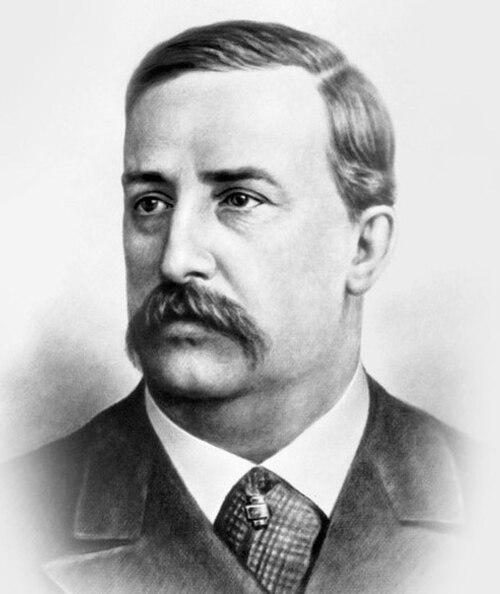
\includegraphics[width=\linewidth]{images/book3/borodin.jpg}
\end{minipage}\hspace{0.02\linewidth}%
\begin{minipage}[t]{0.18\linewidth}
\vspace{0pt}
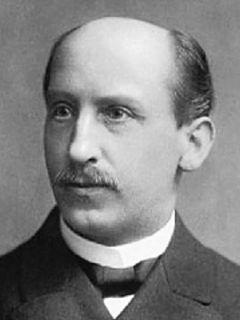
\includegraphics[width=\linewidth]{images/book3/claisen.jpg}
\end{minipage}\hfill
\begin{minipage}[t]{0.58\linewidth}
\vspace{0pt}
\omterm{def:b2:enolates-aldol:aldol}{ऐल्डोल} अभिक्रिया का वर्णन 1872 में शार्ल-अडोल्फ़ वुर्ट्स ने और, स्वतंत्र रूप से, अलेक्सांद्र
बोरोदिन ने किया, जो सेंट पीटर्सबर्ग के रसायनज्ञ थे और आज \textit{प्रिंस इगोर} के संगीतकार के रूप में अधिक जाने जाते हैं।
लुडविग क्लाइज़न ने 1887 में कार्बोनिल यौगिकों के संघननों को एस्टरों तक विस्तारित किया। (चित्र: बोरोदिन,
अज्ञात लेखक, सार्वजनिक अधिकार-क्षेत्र; क्लाइज़न, वेरोनिका॰विलाग्रासा, CC BY-SA 4.0; विकिमीडिया कॉमन्स।)
\end{minipage}
\end{history}

\begin{safety}{\ghs[5mm]{GHS02}\,\ghs[5mm]{GHS05}\,\ghs[5mm]{GHS07}}
सोडियम एथॉक्साइड और लिथियम डाइआइसोप्रोपिलऐमाइड संक्षारक हैं और जल से अभिक्रिया करते हैं; LDA विलयन
ज्वलनशील हैं और अक्रिय गैस के अंतर्गत सँभाले जाते हैं। बेन्ज़ैल्डिहाइड और प्रोपेनोन हानिकारक और ज्वलनशील हैं।
% ledger: ghs:NaOEt, ghs:LDA, ghs:benzaldehyde, ghs:acetone
\end{safety}

\section{अभ्यास}

\begin{exercise}[$\star$]\label{exo:b2:enolates-aldol:1}
ब्यूटेनोन और साइक्लोहेक्सेनोन के \omterm{def:b2:enolates-aldol:tautomerism}{ईनॉल} \omterm{def:b2:enolates-aldol:tautomerism}{चलावयवी} खींचिए।
\end{exercise}

\begin{exercise}[$\star$]\label{exo:b2:enolates-aldol:2}
अपने सबसे अम्लीय \ce{C-H} की अम्लता के क्रम में रखिए: प्रोपेनोन, पेंटेन-2,4-डाइओन, एथिल 3-ऑक्सोब्यूटेनोएट,
एथेन।
\end{exercise}

\begin{exercise}[$\star$]\label{exo:b2:enolates-aldol:3}
सोडियम हाइड्रॉक्साइड के साथ एथेनल का \omterm{def:b2:enolates-aldol:aldol}{ऐल्डोल} और संघनन उत्पाद दीजिए।
\end{exercise}

\begin{exercise}[$\star$]\label{exo:b2:enolates-aldol:4}
हेक्सेनोइक अम्ल का \omterm{def:b2:enolates-aldol:decarboxylation}{मैलोनिक एस्टर संश्लेषण} लिखिए: कौन-सा हैलोऐल्केन चाहिए?
\end{exercise}

\begin{exercise}[$\star\star$]\label{exo:b2:enolates-aldol:5}
2-मेथिलसाइक्लोहेक्सेनोन के गतिक और \omterm{def:b2:enolates-aldol:kinetic-enolate}{ऊष्मागतिक ईनोलेट} खींचिए और वे परिस्थितियाँ बताइए जो
हर एक को देती हैं।
\end{exercise}

\begin{exercise}[$\star\star$]\label{exo:b2:enolates-aldol:6}
प्रोपेनोन के साथ बेन्ज़ैल्डिहाइड (हर एक का एक तुल्यांक) के संकर \omterm{def:b2:enolates-aldol:aldol}{ऐल्डोल संघनन} का उत्पाद दीजिए
और समझाइए कि बेन्ज़ैल्डिहाइड स्वयं से संघनित क्यों नहीं होता।
\end{exercise}

\begin{exercise}[$\star\star$]\label{exo:b2:enolates-aldol:7}
क्षारक में हेक्सेन-2,5-डाइओन अंतःअणुक \omterm{def:b2:enolates-aldol:aldol}{ऐल्डोल संघनन} करता है। कौन-सा वलय बनता है? संभावित वलयों के
बीच चयन को समझाइए।
\end{exercise}

\begin{exercise}[$\star\star$]\label{exo:b2:enolates-aldol:8}
एथिल एथेनोएट का \omterm{def:b2:enolates-aldol:claisen}{क्लाइज़न संघनन} और अम्लीय उपचार-पश्चात् प्रक्रिया के बाद उसका उत्पाद लिखिए।
\end{exercise}

\begin{exercise}[$\star\star$]\label{exo:b2:enolates-aldol:9}
इनमें से कौन-से धनात्मक आयोडोफ़ॉर्म परीक्षण देते हैं: प्रोपेनोन, पेंटेन-3-ओन, एथेनल, ऐसीटोफ़ीनोन?
\end{exercise}

\begin{exercise}[$\star\star\star$]\label{exo:b2:enolates-aldol:10}
डाइएथिल हेक्सेनडाइओएट का डीकमान चक्रीकरण और उत्पाद के वलय का आकार लिखिए।
\end{exercise}

\begin{exercise}[$\star\star\star$]\label{exo:b2:enolates-aldol:11}
(\textit{R})-3-मेथिलपेंटेन-2-ओन तनु सोडियम हाइड्रॉक्साइड में अपनी प्रकाशिक सक्रियता खो देता है, परंतु
(\textit{R})-4-मेथिलहेक्सेन-2-ओन नहीं। समझाइए।
\end{exercise}

\begin{exercise}[$\star\star\star$]\label{exo:b2:enolates-aldol:12}
1,5-डाइफ़ेनिलपेंटा-1,4-डाइईन-3-ओन तक, फिर दो भिन्न ऐरिल समूहों वाले एक डाइईनोन तक एक मार्ग प्रस्तावित कीजिए,
और बताइए कि दूसरा अधिक कठिन क्यों है।
\end{exercise}

\section{समस्या: डाइबेन्ज़ैल्ऐसीटोन}

\begin{problem}[{सप्ताहांत समस्या --- प्रोपेनोन का ईनोलेट और बेन्ज़ैल्डिहाइड की भूमिका, दोनों
ऐल्डोल संघनन, संयुग्मित उत्पाद, और एक निर्माण की रससमीकरणमिति और लब्धि}]
\label{pb:b2:enolates-aldol:1}
निर्माण (अभ्यास के आँकड़े): बेन्ज़ैल्डिहाइड के \qty{2.1}{mL} और प्रोपेनोन के \qty{0.75}{mL} को
एथेनॉल में जलीय सोडियम हाइड्रॉक्साइड के साथ विलोडित किया जाता है; 1,5-डाइफ़ेनिलपेंटा-1,4-डाइईन-3-ओन
(डाइबेन्ज़ैल्ऐसीटोन) के पीले क्रिस्टल अलग होते हैं; लब्धि 75~\%। घनत्व (\unit{g/cm^3}): बेन्ज़ैल्डिहाइड 1.045, प्रोपेनोन 0.7845।
मोलर द्रव्यमान (\unit{g/mol}): C 12.011, H 1.008, O 15.999।
% ledger: rho:benzaldehyde, rho:acetone, aw:C, aw:H, aw:O, ghs:dibenzalacetone

\medskip
\noindent\textbf{भाग I --- भागीदार।}
\begin{enumerate}
  \item किस भागीदार के $\alpha$ हाइड्रोजन हैं? कितने?
  \item प्रोपेनोन का \omterm{def:b2:enolates-aldol:enolate}{ईनोलेट} खींचिए।
  \item बेन्ज़ैल्डिहाइड \omterm{def:b2:enolates-aldol:enolate}{ईनोलेट} क्यों नहीं बना सकता?
  \item प्रोपेनोन स्वयं के बजाय बेन्ज़ैल्डिहाइड से अभिक्रिया क्यों करता है?
  \item ऐल्डिहाइड कीटोन से बेहतर इलेक्ट्रॉनरागी क्यों है?
  \item यहाँ क्षारक के रूप में हाइड्रॉक्साइड पर्याप्त क्यों है?
\end{enumerate}

\medskip
\noindent\textbf{भाग II --- क्रियाविधि।}
\begin{enumerate}[resume]
  \item बेन्ज़ैल्डिहाइड से \omterm{def:b2:enolates-aldol:enolate}{ईनोलेट} का योग लिखिए।
  \item बने \omterm{def:b2:enolates-aldol:aldol}{ऐल्डोल} का निर्जलीकरण लिखिए।
  \item यहाँ निर्जलीकरण आसान क्यों है?
  \item अभिक्रिया दूसरी बार क्यों हो सकती है?
  \item समग्र समीकरण लिखिए।
  \item इस निर्माण में अभिक्रिया को पूर्णता तक क्या ले जाता है?
\end{enumerate}

\medskip
\noindent\textbf{भाग III --- उत्पाद।}
\begin{enumerate}[resume]
  \item डाइबेन्ज़ैल्ऐसीटोन में कितने \ce{C=C} द्वि-आबंध हैं, और (मुख्यतः) किस विन्यास के?
  \item (\textit{E},\textit{E}) समावयवी अनुकूल क्यों है?
  \item संयुग्मित $\pi$ आबंध गिनिए।
  \item यौगिक पीला क्यों है जबकि उसके भागीदार रंगहीन हैं?
  \item क्या डाइबेन्ज़ैल्ऐसीटोन किरैल है?
\end{enumerate}

\medskip
\noindent\textbf{भाग IV --- रससमीकरणमिति और लब्धि।}
\begin{enumerate}[resume]
  \item बेन्ज़ैल्डिहाइड, प्रोपेनोन और डाइबेन्ज़ैल्ऐसीटोन के मोलर द्रव्यमान परिकलित कीजिए।
  \item दोनों अभिकर्मकों की मात्राएँ परिकलित कीजिए।
  \item कौन-सा अभिकर्मक सीमांत है?
  \item उत्पाद का सैद्धांतिक द्रव्यमान परिकलित कीजिए।
  \item प्रोपेनोन के आधिक्य की तुलना में बेन्ज़ैल्डिहाइड का हल्का आधिक्य बेहतर क्यों है?
  \item प्रोपेनोन का आधिक्य क्या देता?
  \item 75~\% लब्धि पर प्राप्त डाइबेन्ज़ैल्ऐसीटोन का द्रव्यमान बताइए।
\end{enumerate}
\end{problem}
